% Copyright (C) 2005-2015 Airbus - EDF - IMACS - Phimeca
% Permission is granted to copy, distribute and/or modify this document
% under the terms of the GNU Free Documentation License, Version 1.2
% or any later version published by the Free Software Foundation;
% with no Invariant Sections, no Front-Cover Texts, and no Back-Cover
% Texts.  A copy of the license is included in the section entitled "GNU
% Free Documentation License".
\renewcommand{\filename}{docUC_InputWithData_KernelSmoothing.tex}
\renewcommand{\filetitle}{UC : PDF fitting by kernel smoothing and graphical validation : superposition of the empirical and kernel smoothing CDF}

% \HeaderNNIILevel
% \HeaderIILevel
\HeaderIIILevel


\index{Distribution!Kernel mixture}
\index{Fitting Distribution!Kernel smoothing}
\index{Graph!Empirical cumulative density function}
\index{Graph!PDF-CDF curves}
\index{Graph!Superposition empirical - kernel smoothed CDF}

The objective of this Use Case is to model the PDF of a random  vector, described by a numerical sample thanks to the kernel smoothing method and to superpose on the same graph the kernel smoothing PDF and the histogram built from the same numerical sample.\\



Details on the kernel smoothing method may be found in the Reference Guide (\extref{ReferenceGuide}{see file Reference Guide - Step B -- Kernel Smoothing}{stepB}).\\


In dimension 1, the kernel smoothed probability density function $\hat{p}$ has the following expression, where $K$ is the univariate kernel, $n$ the numerical sample size and $(X_1, \cdots, X_n) \in \Rset^n$ the univariate random sample with $\forall i, \, \, X_i \in \Rset$ :
\begin{equation}
  \label{kernelSmooth}
  \hat{p}(x) = \displaystyle \frac{1}{nh}\sum_{i=1}^{n} K\left(\frac{x-X_i}{h}\right)
\end{equation}
The kernel $K$ is a function satisfying $\int K(x)\, dx=1$. Usually, $K$ is chosen to be a unimodal probability density function that is symmetric about 0.\\
The parameter $h$ is called the \emph{bandwidth}.\\

 In dimension $d>1$, OpenTURNS uses the product kernel $K_d$, defined by: 
  \begin{align*}
    K_d(\vect{x}) = \displaystyle \prod_{j=1}^{d} K(x_j)
  \end{align*}
 where $\vect{x} = (x_1, \cdots, x_d)\in \Rset^d$. Thus, the kernel smoothed probability density function in dimension $d$ writes:
  \begin{align*}
    \hat{p}(\vect{x}) = \displaystyle \frac{1}{N \prod_{j=1}^{d}h_j} \sum_{i=1}^{N} K_d\left(\frac{x_1 - X_{i1} }{h_1}, \dots, \frac{x_d - X_{id}}{h_d}\right)
  \end{align*}
where $(\vect{X}_1, \cdots, \vect{X}_n)$ is the d-variate random  sample which components are denoted $\vect{X}_i = (X_{i1}, \dots, X_{id})$. \\
  Let's note that the bandwidth is the vector $\vect{h} = (h_1, \cdots, h_d)$. \\
The default kernel of OpenTURNS is the product of standard Normal distributions. The dimension of the product is automatically evaluated from the random sample.\\

In dimension 1, the boundary effects may be taken into account in OpenTURNS : the boundaries are automatically detected from the numerical sample (with the \textit{min} and \textit{max} functions) and the kernel smoothed PDF is corrected in the boundary areas to remain within the boundaries, according to the miroring technique :
\begin{itemize}
\item the Scott bandwidth is evaluated from the numerical sample : $h$
\item two subsamples are extracted from the inital numerical sample, containing all the points within the range $[min, min + h[$ and  $]max-h, max]$,
\item both subsamples are transformed into their symmetric samples with respect their respective boundary : its results two samples within the range  $]min-h, min]$ and  $[max, max+h[$,
      \item a kernel smoothed PDF is built from the new numerical sample composed with the initial one and the two new ones, with the previous bandwidth $h$,
      \item this last kernel smoothed PDF is truncated within the inital range  $[min, max]$ (conditional PDF).
\end{itemize}
\vspace*{0.1cm}

The choice of the kind of the kernel is free in OpenTURNS : it is possible to select any 1D distribution and to define it as a kernel. However, in order to optimize the efficiency of the kernel smoothing fitting (it means to minimise the AMISE error), it is recommended to select a {\bf symmetric distribution} for the kernel. \\
All the distribution default constructors of OpenTURNS create a symmetric default distribution when possible. It is also possible to work with the Epanechnikov kernel, which is a $Beta(r=2, t=4, a=-1, b=1)$. \\

The bandwidth $\vect{h}$ may be fixed by the User. However, it is recommended to let OpenTURNS evaluate it automatically from the numerical sample according to the following rules :
\begin{itemize}
\item In dimension $d$, OpenTURNS automatically applies the Scott rule.
\item In dimension 1, the automatic bandwidth selection method depends  on the size $n$ of the numerical sample. As a matter of fact, the computation bottleneck is the estimation of the estimators $\hat{\Phi}_r$ as it requires the evaluation of a double summation on the numerical sample, which has a cost of $\cO(n^2)$.
  \begin{itemize}
  \item if $n \leq 250$, the Solve-the-equation  plug-in method is used on the entire numerical sample.
  \item if $n>250$, the Solve-the-equation  plug-in method is too computationnally expensive. Then, OpenTURNS proceeds as follows :the plug-in method on the entire numerical sample if its size is inferior to 250; the mixted method in the other case. Refer to the Reference Guide for more details on these methods.
  \end{itemize}
\end{itemize}


It is possible to specify a particular bandwidth, evaluated according to one of the previous rules as follows :
\begin{itemize}
\item \emph{computeSilvermanBandwidth} applies the Silverman rule,
\item \emph{computePluginBandwidth} applies the plug-in method on the entire numerical sample,
\item \emph{computeMixedBandwidth} applies the mixted plug-in method on the entire numerical sample, as described above.
\end{itemize}

\textspace\\
\requirements{
  \begin{description}
  \item[$\bullet$] a nD-sample : {\itshape sample}
  \item[type:]  NumericalSample
  \end{description}
}
             {
               \begin{description}
               \item[$\bullet$] a kernel smoothed distribution : {\itshape kernelSmoothedDist}
               \item[type:]  Distribution
               \end{description}
             }

             \textspace\\
             Python script for this UseCase :

             \inputscript{script_docUC_InputWithData_KernelSmoothing}

             \textspace\\


             Figures \ref{pdf_KernelSmooth} and \ref{cdf_KernelSmooth}  show a 1D kernel smoothing of a distribution of type Mixture which PDF is defined by : 0.2*Triangular(1.0, 2.0, 4.0) + 0.5*Normal(-1.0, 1.0) + 0.3*Exponential(1.0, 3.0), thanks to a numerical sample of size $10^4$, with a Normal,  Triangular and Epanechnikov kernel, when the  bandwidth is selected according to the mixted plug-in method.\\

             Figures \ref{pdf_KernelSmoothBWSel} and \ref{cdf_KernelSmoothBWSel} show the difference when the previous distribution is estimated with  a Normal kernel and when the bandwidth is selected according to the Silverman rule, the plug-in method or the mixted plug-in method, thanks to a numerical sample of size $10^3$.\\

             Figures \ref{pdf_KernelSmooth_boundary} and \ref{cdf_KernelSmooth_boundary} show the effect of the boundary treatment in the kernel smoothing through the example of the exponential distribution $Exp(\lambda = 2.0, \gamma = 0.0)$. A Normal kernel is used and the  bandwidth is selected according to the mixted plug-in method, thanks to a numerical sample of size $10^4$.


             \begin{figure}[H]
               \begin{minipage}{7cm}
                 \begin{center}
                   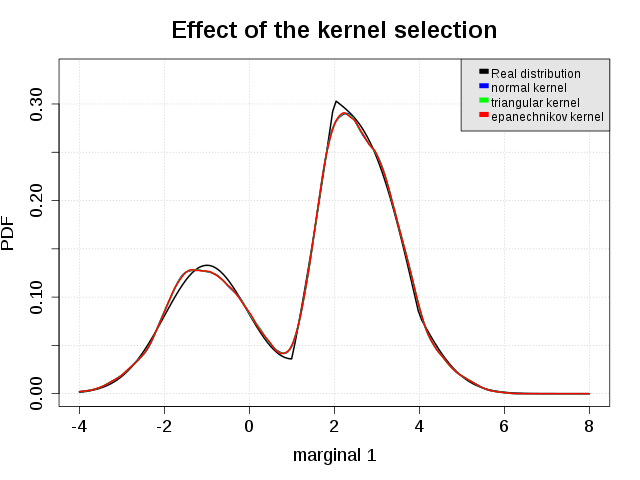
\includegraphics[width=7cm]{Figures/kernelSmoothing_pdf.png}
                   \caption{PDF of th kernel smoothed distribution and of the real one with different kernels.}
                   \label{pdf_KernelSmooth}
                 \end{center}
               \end{minipage}
               \hfill
               \begin{minipage}{7cm}
                 \begin{center}
                   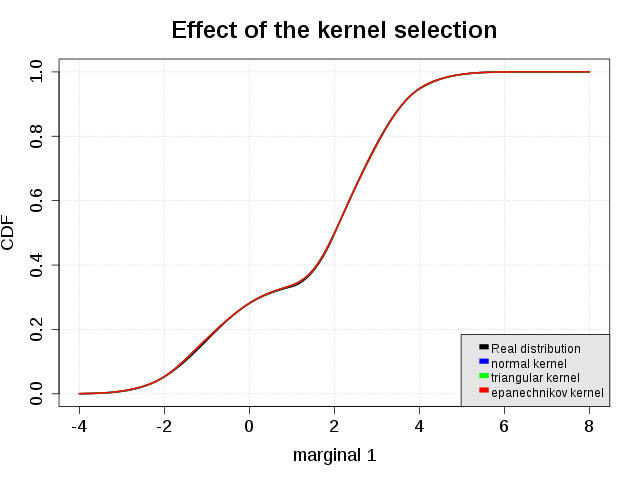
\includegraphics[width=7cm]{Figures/kernelSmoothing_cdf.png}
                   \caption{CDF of the kernel smoothed distribution and of the real one with different kernels.}
                   \label{cdf_KernelSmooth}
                 \end{center}
               \end{minipage}
             \end{figure}


             \begin{figure}[H]
               \begin{minipage}{7cm}
                 \begin{center}
                   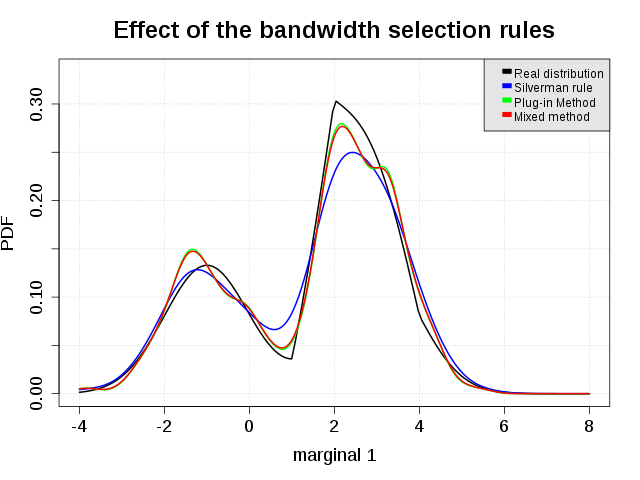
\includegraphics[width=7cm]{Figures/kernelSmoothingBWSel_pdf.png}
                   \caption{PDF of the kernel smoothed distribution and of the real one with different bandwidth selection rules.}
                   \label{pdf_KernelSmoothBWSel}
                 \end{center}
               \end{minipage}
               \hfill
               \begin{minipage}{7cm}
                 \begin{center}
                   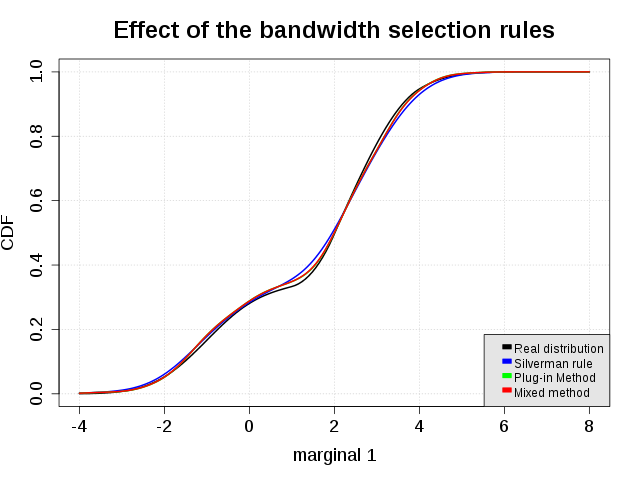
\includegraphics[width=7cm]{Figures/kernelSmoothingBWSel_cdf.png}
                   \caption{CDF of the kernel smoothing distributions and of the real one with different bandwidth selection rules.}
                   \label{cdf_KernelSmoothBWSel}
                 \end{center}
               \end{minipage}
             \end{figure}

             \begin{figure}[H]
               \begin{minipage}{7cm}
                 \begin{center}
                   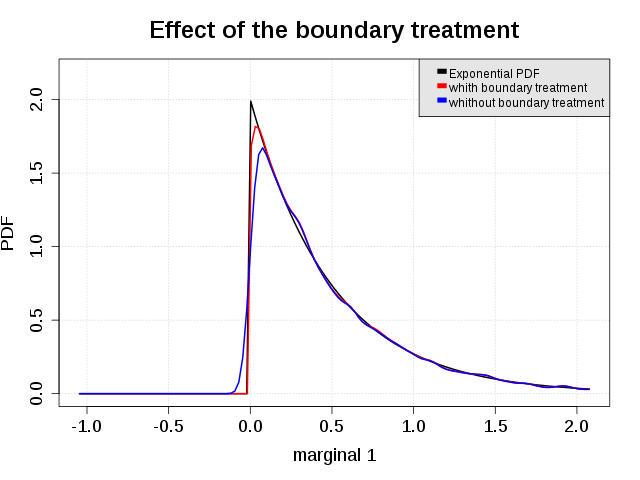
\includegraphics[width=7cm]{Figures/kernelSmoothing_boundary_pdf.png}
                   \caption{Effect of the boundary treatment on the kernel smoothing PDF of an exponential distribution.}
                   \label{pdf_KernelSmooth_boundary}
                 \end{center}
               \end{minipage}
               \hfill
               \begin{minipage}{7cm}
                 \begin{center}
                   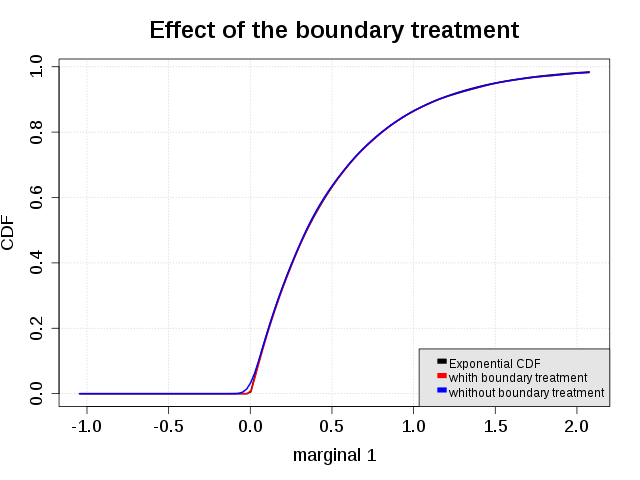
\includegraphics[width=7cm]{Figures/kernelSmoothing_boundary_cdf.png}
                   \caption{Effect of the boundary treatment on the kernel smoothing CDF of an exponential distribution.}
                   \label{cdf_KernelSmooth_boundary}
                 \end{center}
               \end{minipage}
             \end{figure}
